% ********** Chapter 1 **********
\section{Design}
\label{sec:chap1:design}

Eine JSR 223-Implementierung f"ur PHP besteht gezwungenermassen aus zwei Teilen: Zum einen einem Java-Teil, welcher im Wesentlichen
die ScriptEngineFactory enth"alt. Dieser ist komplett in Java ohne die Verwendung von nativen (JNI-) Aufrufen implementiert und
deckt s"amtliche Funktionalit"at des Auffindungsmechanismus ab. Zum anderen einem nativen Teil, welcher aus 
einem C- oder C++ - Programm, das die n"otigen Aufrufe an PHP vornimmt, besteht.
Die eigentliche ScriptEngine verbindet diese beiden Teile, indem sie aus Java heraus dieses in nativen Code "ubersetzte 
Programm mittels JNI anspricht.
Um allerdings JSR 223 "uberhaupt nutzen zu k"onnen, m"ussen alle Klassen aus dem Package \texttt{javax.script}
im Java-Classpath liegen, damit dem Anwender der Zugriff auf die ScriptEngine "uber den ScriptEngineManager m"oglich ist.
Hierzu kann entweder eine Java-Runtime der Version 6 oder aber eine eigene Implementierung dieser Klassen genutzt werden. 
Die im folgenden beschriebene JSR 223 Implementierung tr"agt den Namen "'Turpitude"'.

\subsection{Java-Teil}
\label{sec:chap1:design:java}

Eine JSR 223-Implementierung muss sich um f"ur den ScriptEngineManager auffindbar zu sein gem"a\ss\ der 
\emph{Jar File Specification} \cite{JARSPEC} als sogenannter \emph{Service Provider}\footnote{
Ein \emph{Service Provider} ist eine spezifische Implementierung eines Interfaces oder einer abstrakten Klasse
} registrieren. Hierzu muss sich im Verzeichnis \texttt{META-INF/services} des Archivs eine Datei
mit dem Namen der Service-Klasse (in diesem Fall \texttt{ScriptEngineFactory}) befinden, in welcher verf"ugbare 
ScriptEngineFactories zeilenweise aufgelistet werden.

Das Package \texttt{net.xp\_framework.turpitude} enth"alt alle Klassen der Implementierung. 
Die ScriptEngineFactory-Implementierung hei\ss t \texttt{PHPScriptEngineFactory} und implementiert direkt das Interface 
\texttt{ScriptEngineFactory} aus \texttt{javax.script}. Im Gegensatz dazu implementiert die Klasse \texttt{PHPScriptEngine} nicht
direkt das Interface \texttt{ScriptEngine}, sondern erbt von der abstrakten Klasse \texttt{AbstractScriptEngine}. Diese bringt f"ur
viele Varianten der \texttt{eval()}-Methode schon eine Realisierung, sowie mit der Klasse \texttt{SimpleScriptContext} schon einen 
\texttt{ScriptContext} mit. Um den "ubergebenen Skriptcode tats"achlich auszuf"uhren, muss dieser an den mittels der Java-Methode
\texttt{System.loadLibary()} geladenen nativen Teil der Implementierung weitergegeben werden. Die Kommunikation mit diesem
nativen Teil findet mittels JNI-Methoden statt.
Weiterhin implementiert die PHPScriptEngine die beiden in \texttt{javax.script} enthaltenen Interfaces \texttt{Compilable} und
\texttt{Invocable}, deren Funktionalit"at zur Erff"ullung einiger der Use-Cases ben"otigt wird. F"ur die Methoden aus
Compilable wird noch eine weitere Klasse - \texttt{PHPCompiledScript} - erstellt, welche direkt von der abstrakten
Klasse \texttt{javax.script.CompiledScript} erbt.
Der Standard schreibt zwar vor, dass die ScriptEngine das Interface Invocable implementiert, allerdings ergibt das aus Sicht
des Autors nur wenig Sinn. Es bleibt unklar auf welchem der "ubersetzten Skripte Methoden und Funktionen aufgerufen werden sollen.
Aus diesem Grund wird neben der \texttt{PHPScriptEngine} auch das \texttt{PHPCompiledScript} dieses Interface implementieren
und Aufrufe der Interfacemethoden bei der \texttt{PHPScriptEngine} werden an das zuletzt "ubersetzte Script weitergeleitet.

Die Kommunikation zwischen Java und PHP findet "uber zwei unterschiedliche Kan"ale statt:
Bei der R"uckgabe von Daten aus einem PHP-Skript werden diese einfach kopiert, wobei primitive Datentypen (bool, long, double und string)
einfach in ihre Java-"Aquivalente (java.lang.Boolean, java.lang.Long, java.lang.Double und java.lang.String) umgesetzt werden.
Da alle Arrays in PHP assoziativer Natur sind, werden sie als untypisierte \texttt{java.util.HashMap} zur"uckgegeben, was bedeutet dass sowohl 
Schl"ussel als auch Wert vom Typ \texttt{java.lang.Object} sind. Einzig f"ur PHP-Objekte wird eine gesonderte Java-Klasse ben"otigt: \texttt{PHPObject}.
Sie enth"alt neben dem Klassennamen auch alle Eigenschaften eines PHP-Objektes. 
Diese werden in einer HashMap gespeichert, mit dem Namen der Eigenschaft als Schl"ussel.
\begin{floatingtable}{
\begin{tabular}{|l|l|}
\hline
Java-Typ & PHP-Typ\\
\hline\hline
jlong & long\\
jint & long\\
jshort & long\\
jchar & long\\
jbyte & long\\
jboolean & bool\\
jfloat & double\\
jdouble & double\\
jstring & string\\
jobject & TurpitudeJavaObject\\
jclass & TurpitudeJavaClass\\
type[] & TurpitudeJavaArray\\
\hline
\end{tabular}}
\caption{Typkonversion Java nach PHP}
\end{floatingtable}
Leider l"asstdie JSR 223-Spezifikation sehr viele Fragen unbeantwortet, so wird beispielsweise zur Typkonversion nur lapidar auf 
Implementierungsdetails verwiesen. Da der Datenaustausch zwischen PHP und Java allerdings einen nicht unwesentlichen Bestandteil
einer JSR223-Implemenation darstellt, muss gezwungenerma\ss en eine Konvention gefunden werden. Diese wird in den Tabellen 4.1 und 4.2
erl"autert, sowohl von Java nach PHP als auch umgekehrt. Weiterhin wird bei der Typkonversion von PHP nach Java zwischen 
Methodenaufrufen und Werter"uckgaben unterschieden. Bei Methodenaufrufen wird versucht, in simple Datentypen wie \texttt{int} und \texttt{double}
umzuwandeln. Weil der aber Standard oft verlangt dass Objekte zur"uckgegeben werden, wird bei der R"uckgabe von Werten in den entsprechenden
Objektyp wie zum Beispiel \texttt{java.lang.Boolean} konvertiert. Einige Java-Klassen und PHP-Objekte werden speziell konvertiert was
in den Tabellen gesondert aufgef"uhrt ist. Beispielsweise wird der
\texttt{java.lang.String} nicht zu einem \texttt{TurpitudeJavaObject}, sondern zu einem String in PHP. Die
Tabellen enthalten auch Verweise auf spezielle PHP-Klassen, die sp"ater im Kapitel \ref{sec:chap1:design:native} erl"autert werden.

\begin{table}
\begin{tabular}[tbh]{|l|l|l|}
\hline
PHP-Typ & Methodenaufruf & Werter"uckgabe\\
\hline\hline
long & jlong & java.lang.Long \\
double & jdouble & java.lang.Double \\
bool & jboolean  & java.lang.Boolean \\
array & java.util.HashTable & java.util.HashTable \\
object & PHPObject & PHPObject\\
constant & jstring & jstring\\
string & jstring & jstring \\
TurpitudeJavaClass & jclass & jstring\\
TurpitudeJavaObject & jobject & jobject\\
TurpitudeJavaArray & jarray & jarray\\
\hline
\end{tabular}
\caption{Typkonversion PHP nach Java, Methodenaufruf und Werter"uckgabe}
\end{table}

Die Eingabe von Daten aus Java heraus in ein PHP-Skript geschieht - gem"a\ss\ der JSR223-Spezifikation - mittels des Kontextes der
ScriptEngine. Hierzu wird dieser - zusammen mit einigen Umgebungsvariablen und -informationen - in eine globale Variable injiziert,
deren Name sich in der ScriptEngine setzen l"asst. Im Unterschied zu den oben beschriebenen R"uckgabewerten stellen die Kontext-Objekte
Referenzen dar, weshalb sich "Anderungen an diesen unmittelbar auf die entsprechenden Java-Objekte auswirken.

Die Abbildung \ref{fig:jsr223impl} zeigt die beteiligten Klassen und ihre Abh"anigkeiten untereinander,
zusammen mit einigen wichtigen Methoden und Attributen. 

\begin{figure}[h]
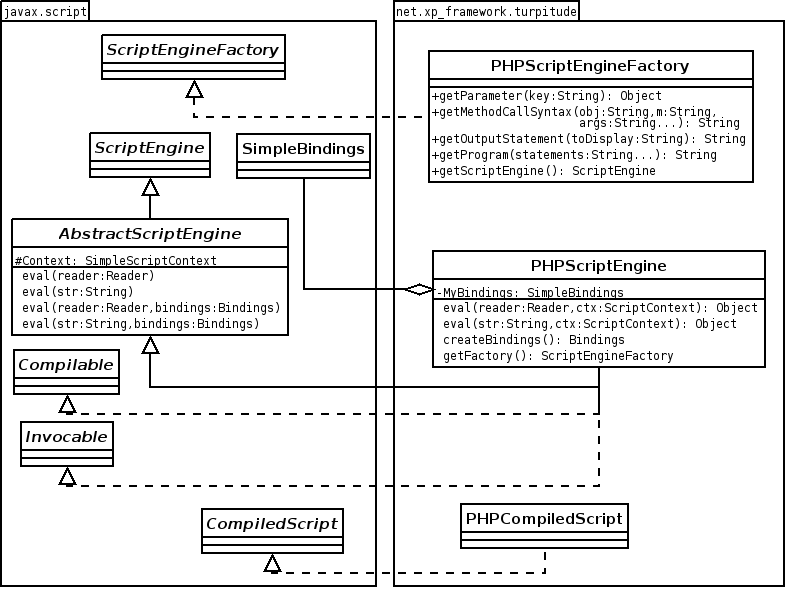
\includegraphics[width=\textwidth]{chap1/img/turpitude.png}
\caption{JSR 223 Implementierung - Architektur}
\label{fig:jsr223impl}
\end{figure}

Der JSR 223 spezifiziert lediglich eine einzige Exception (\texttt{ScriptException}) um alle m"oglichen Laufzeitfehler innerhalb einer 
Implementierung abzudecken. Um dem Anwender trotzdem eine M"oglichkeit einer differenzierten Fehlerauswertung zu geben, werden drei
zus"atzliche Exceptions eingef"uhrt: die \texttt{PHPScriptException}, die \texttt{PHPCompileException} und die \texttt{PHPEvalException} 
(siehe Abbildung \ref{fig:jsr223exceptions}). Die \texttt{PHPScriptException} dient zum Einen als Oberklasse, zum anderen kann der Anwender durch 
sie erkennen, ob das aufgetretene Problem implementationsspezifisch ist. Die beiden anderen neuen Exceptions werden genutzt um Fehler 
beim "Ubersetzen (\texttt{PHPCompileException}) oder beim Ausf"uhren (\texttt{PHPEvalException}) eines Skripts voneinander abzugrenzen.

\begin{figure}[h]
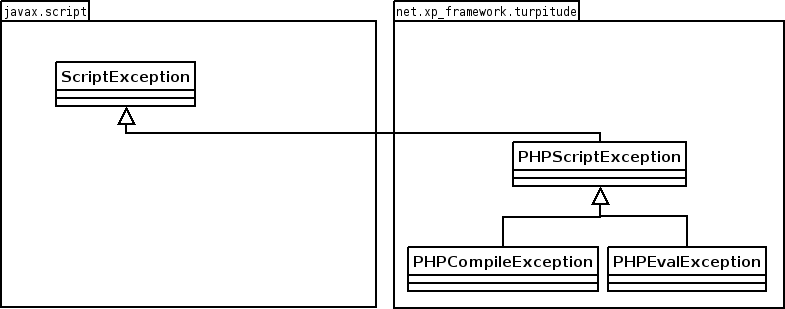
\includegraphics[width=\textwidth]{chap1/img/exceptions.png}
\caption{JSR 223 Implementierung - Exceptions}
\label{fig:jsr223exceptions}
\end{figure}

\subsection{Nativer/PHP-Teil}
\label{sec:chap1:design:native}

Der native Teil der Implementierung teilt sich wiederum auf in JNI-Methoden, f"ur welche die Headerdateien automatisch aus
der Java-Klasse der PHPScriptEngine generiert werden k"onnen, und in die Implementierung einer SAPI. Hierzu muss im
Wesentlichen ein sogenanntes \texttt{sapi\_module\_struct} angelegt und bef"ullt werden, welches neben einigen Strings
haupts"achlich Funktionspointer auf R"uckruffunktionen enth"alt, welche vom PHP-Interpreter aufgerufen werden. Da es
kaum m"oglich ist, dieses Konstrukt sinnvoll in eine objektorientierte Architektur einzuf"ugen, wird auf eine solche
vollst"andig verzichtet. Das \texttt{sapi\_module\_struct} und die dazugeh"origen Funktionen werden auf traditionelle,
prozedurale Art und Weise implementiert.

Die zu implementierenden SAPI-Funktionen ergeben sich aus den Anforderungen der Zend-API und sollen an dieser Stelle nur
sehr kurz erl"autert werden: die Funktionen \texttt{turpitude\_read\_cookies}, \texttt{turpitude\_flush}, \texttt{turpitude\_send\_headers},
\texttt{turpitude\_send\_header} und \texttt{turpitude\_log\_message} k"onnen leer, beziehungsweise auf triviale Art und Weise
implementiert werden, da sie f"ur den geplanten Einsatz der PHP-Umgebung keine Relevanz haben. Die Funktionen
\texttt{turpitude\_startup} und \texttt{turpitude\_register\_variables} leiten den Aufruf einfach an die entsprechenden
Zend-API Funktionen \texttt{php\_module\_startup} respektive \texttt{php\_import\_environment\_ variables} weiter, lediglich
die Funktion \texttt{turpitude\_error\_cb}, welche die R"uckruffunktion f"ur PHP-Laufzeitfehler darstellt, bedarf einer
komplizierteren Implementierung, da sie den PHP-Fehler als passende Java-Exception an den Anwender weitergeben soll.

Die JNI-Methoden ergeben sich aus dem Java-Quelltext, da sie Implementierungen von in Java als \texttt{native} deklarierten 
Methoden darstellen. Ihre Hauptaufgabe ist das Ausf"uhren von PHP-Quelltext beziehungsweise von PHP-Anweisungen.
Ausnahmen bilden lediglich die Methoden \texttt{startUp()} und \texttt{shutDown()} der PHPScriptEngine, welche
die Initialisierung beziehungsweise die kontrollierten Dekonstruktion der PHP-Laufzeitunmgebung und er Turpitude-spezifischen
Klassen "ubernehmen.

Um die Implementierung in PHP nutzen zu k"onnen muss auch hier eine Schnittstelle geschaffen werden. Leider schreibt
die Spezifikation keine API f"ur die Skriptseite vor, was zu einer Nichtaustauschbarkeit der Implementierung f"uhren kann.
Nichtsdestotrotz werden auf PHP-Seite folgende Klassen eingef"uhrt, welche im Wesentlichen JNI-Funktionen abbilden, und
in vielen F"allen auch die JNI-Syntax, zum Beispiel f"ur Java-Methoden, verwenden:

\textbf{TurpitudeEnvironment} - bietet neben der Methode \texttt{getScriptContext()}, die den JSR223 ScriptContext zur"uckgibt,
auch Schnittstellen an um grundlegende Java-Funktionalit"at aus PHP heraus anzusprechen:
\texttt{FindClass()} erzeugt die Repr"asentation einer Java-Klasse in PHP, \texttt{instanceOf()} "uberpr"uft, ob ein Java-Objekt 
Instanz einer bestimmten Java-Klasse ist. Weiterhin werden mit \texttt{throw()}, \texttt{throwNew()}, \texttt{exceptionOccurred()} und 
\texttt{exceptionClear()} Methoden angeboten, um Java-Exceptions zu werfen und zu fangen. TurpitudeEnvironment implementiert
das bekannte \emph{Singleton-Entwurfsmuster}, kann also nicht mehrfach existieren und wird zus"atzlich unter einem konfigurierbaren
Namen in das PHP-Superglobal\footnote{
Superglobals sind Variablen, auf die innerhalb eines PHP-Skriptes aus jedem Scope heraus zugegriffen werden kann. Superglobals k"onnen
nicht vom PHP-Anwender erzeugt werden, sondern werden von der PHP-Laufzeitunmgebung verwaltet.
} \texttt{\$\_SERVER} eingef"uhrt, in welchem laut dem PHP-Manual \cite{PHPMAN} SAPI-Informationen "uber die
Laufzeitumgebung gespeichert werden sollen.

\textbf{TurpitudeJavaClass} - PHP-Repr"asentation einer Java-Klasse, wird mittels der Methode \texttt{TurpitudeEnvironment::findClass()} erzeugt.
Bietet mit \texttt{findMethod()}, \texttt{findStaticMethod()} und \texttt{findConstructor()} M"oglichkeiten um gew"ohnliche Methoden, statische
Methoden und Konstruktoren der repr"asentierten Java-Klasse zu erzeugen. Weiterhin k"onnen mittels der Methode \texttt{create()} Instanzen
der Klasse erzeugt, und mittels der Methode \texttt{invokeStatic()} k"onnen statische Methoden der Klasse aufgerufen werden.
Enth"alt als Attribut den JNI-formatierten Klassennamen. 

\textbf{TurpitudeJavaMethod} - bildet eine Java-Methode in PHP ab. TurpitudeJavaMethod bietet selbst keine 
f"ur den Anwender aufrufbaren Methoden an und wird nur
als Parameter f"ur \texttt{TurpitudeJavaClass::create()} und beim Methodenaufruf auf Objekten und Klassen ben"otigt.
Als Attribute werden der Methodenname, deren Signatur sowie ein Indikator, ob die Methode statisch aufgerufen werden kann, vorgehalten.

\textbf{TurpitudeJavaObject} - repr"asentiert ein Java-Objekt, wird mittels der Methode \texttt{TurpitudeJavaClass::create()} erzeugt. Neben Methoden
die den sowohl lesenden als auch schreibenden Zugriff auf Attribute der Java-Klasse erlauben (\texttt{javaGet()} und \texttt{javaSet()}), k"onnen
auch direkt Methoden des gekapselten Java-Objektes mittels \texttt{javaInvoke()} aufgerufen werden. Falls m"oglich soll der Methodenaufruf aber
intuitiv nach folgendem Schema erlaubt werden:
\begin{lstlisting}[caption=angestrebte Syntax zum Aufruf von Java-Methoden in PHP]
$object->method($param1, $param2, ...);
\end{lstlisting}
R"uckgabewerte von Methodenaufrufen werden entweder auf skalare Typen in PHP oder wieder als TurpitudeJavaObject-Objekte abgebildet.
Eine Besonderheit bilden allerdings Java-Arrays: Diese k"onnten zwar als einfache Java-Objekte abgebildet werden, allerdings w"urde das 
nur den Zugriff auf Attribute erlauben, die allen Java-Arrays gemeinsam sind - wie beispielsweise \texttt{length}. Folglich muss eine weitere
Klasse eingef"uhrt werden, um dem Anwender auch den Zugriff auf die Elemente eines Java-Arrays zu erm"oglichen:

\textbf{TurpitudeJavaArray} - erlaubt den direkten Zugriff auf Elemente eines Java-Arrays in PHP. Allerdings k"onnen keine neuen Eintr"age
erzeugt werden, da Java-Arrays - anders als PHP-Arrays - nicht als HashMap, sondern als "'echte"' Arrays im Speicher abgebildet
sind, und eine Erweiterung dieses Bereiches nicht ohne Weiteres m"oglich ist. Der Zugriff auf diese Arrays soll nicht nur "uber 
Funktionen wie \texttt{get()} und \texttt{set()}, sondern auch "uber den Klammern-Operator [ ] m"oglich sein, um den Anwender einen
intuitiven Umgang zu bieten. Au\ss erdem soll das iterieren "uber Java-Arrays sowohl "uber die objektorientierte, in PHP5
enthaltene Schnittstelle \texttt{Iterator}, als auch "uber den normalen PHP-Operator \texttt{foreach} m"oglich sein. Das
\texttt{TurpitudeJavaArray} implementiert das PHP-Interface \texttt{IteratorAggregate}.

\textbf{TurpitudeJavaArrayIterator} - erlaubt das Iterieren "uber Java-Arrays in PHP. Der \texttt{TurpitudeJavaArrayIterator} implementiert
das PHP-Interface \texttt{Iterator} um das objektorientierte Iterieren "uber Java-Arrays zu erm"oglichen. Intern wird die aktuelle
Position im Array in einer einfachen Z"ahlvariable gespeichert. Wird diese gr"o\ss er oder gleich der L"ange des Java-Arrays wird der
Iterator ung"ultig und muss mittels \texttt{rewind()} zur"uckgesetzt werden. \texttt{next()} inkrementiert diesen Z"ahler um eins, die Methoden
\texttt{current()} und \texttt{key()} liefern das aktuelle Element beziehungsweise die aktuelle Position.

Der Zusammenhang zwischen Java-Arrays, den Turpitude-Klassen und PHP-Interfaces ist in der Abbilding \ref{fig:javaarrays} dargestellt.
Das von Java bereitgestellte Array wird in PHP in einem \texttt{TurpitudeJavaArray} gekapselt. Ein Aufruf der Methode
\texttt{getIterator()} erzeugt einen \texttt{TurpitudeJavaArrayIterator}, der intern eine Referenz auf das \texttt{TurpitudeJavaArray}
vorh"alt. 

\begin{figure}[h]
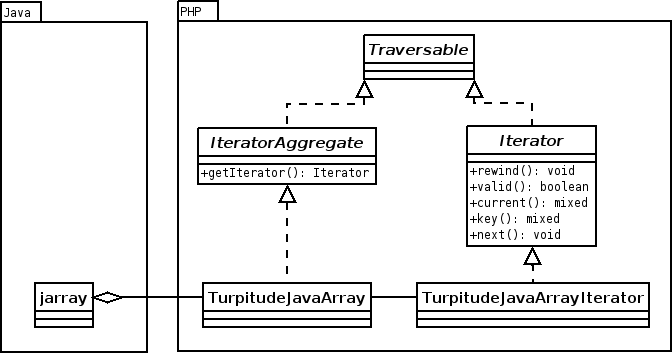
\includegraphics[width=\textwidth]{chap1/img/javaarrays.png}
\caption{Java-Arrays in PHP}
\label{fig:javaarrays}
\end{figure}

Ein typischer Ablauf eines PHP-Skriptes, welches auf Java-Objekte und Methoden zugreift, soll wie in Abbildung \ref{fig:phpseq} aufgezeigt 
aussehen:
Das \texttt{TurpitudeEnvironment} besteht "uber die komplette Laufzeit des Skriptes. Der Anwender erzeugt mittels der Methode \texttt{findClass()} 
des \texttt{TurpitudeEnvironment} eine \texttt{TurpitudeJavaClass} und ruft auf dieser die Methode \texttt{findConstructor()} auf, welche ihm 
eine Instanz der Klasse \texttt{TurpitudeJavaMethod} zur"uckgibt. Diese wiederum 
kann der Anwender der TurpitudeJavaClass beim Aufruf von \texttt{create()} "ubergeben, um schlussendlich eine Instanz der Klasse zu erzeugen.
Um nun auf dem Java-Objekt eine Methode aufzurufen, muss diese zun"achst wieder per \texttt{findMethod()} erzeugt werden, um dann der
Methode \texttt{javaInvoke()} zusammen mit den geforderten Parametern "ubergeben zu werden.

\begin{figure}[h]
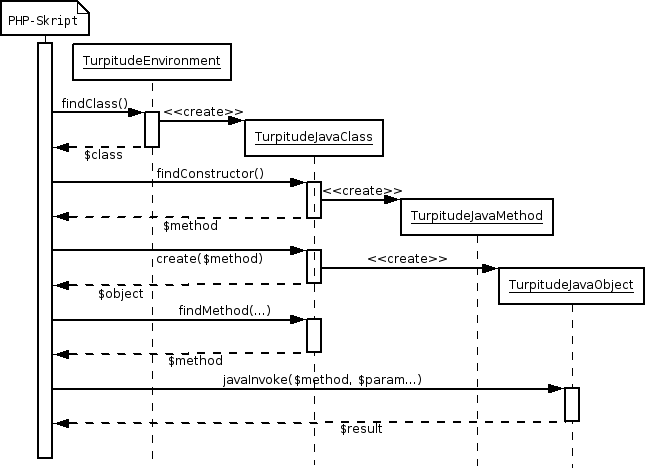
\includegraphics[width=\textwidth]{chap1/img/phpseq.png}
\caption{Ablauf eines PHP-Skriptes mit Zugriff auf Java-Objekte}
\label{fig:phpseq}
\end{figure}



% ********** End of chapter **********
